%==========================================================
%  CHAPITRE 4 — Réalisation du deuxième sprint
%==========================================================
\chapter{Réalisation du deuxième sprint}
\label{Chapitre_4}

{\Large\textbf{Sprint : Gérer les processus des réservations}}

%----------------------------------------------------------
\section{Introduction}
\label{Chapitre4_Introduction}

En se basant sur la planification établie dans le chapitre précédent, ce chapitre est
consacré à la réalisation du Sprint 2. Nous aborderons successivement la description
fonctionnelle, la conception, ainsi que les diagrammes de séquence et de classe
associés aux fonctionnalités développées au cours de ce sprint. Ces fonctionnalités
concernent principalement la gestion des réservations, le suivi du score client, le
traitement des réclamations, la consultation des statistiques et la gestion des messages.

%----------------------------------------------------------
\section{Backlog produit du deuxième sprint}
\label{sec:backlog_sprint2}

\begin{table}[H]
\centering
\caption{Backlog produit du deuxième sprint}
\label{tab:backlog-sprint2}
\renewcommand{\arraystretch}{1.4}
\resizebox{\textwidth}{!}{
\begin{tabular}{|l|c|l|p{4cm}|p{5cm}|c|}
\hline
\textbf{Acteur} & \textbf{ID} & \textbf{Thème} & \textbf{User Story} & \textbf{Tâche} & \textbf{Estimation (Jours)} \\
\hline

\multirow{2}{*}{Internaute}
& US15 & Interagir avec chatbot 
& Interagir avec le chatbot
& Intégrer le module chatbot. & \multirow{2}{*}{4} \\
\cline{5-5}
& & & & Tester. & \\
\hline

\multirow{4}{*}{Client}
& US09 & Effectuer réservation 
& Effectuer une réservation
& Implémenter la réservation d'un véhicule. & \multirow{2}{*}{5} \\
\cline{5-5}
& & & & Tester. & \\
\cline{2-6}

& US10 & Consulter réservations en cours 
& Consulter les réservations en cours
& Implémenter la consultation des réservations. & \multirow{2}{*}{4} \\
\cline{5-5}
& & & & Tester. & \\
\hline

\multirow{4}{*}{Agence}
& US11 & Traiter réservations et reclamations 
& Traiter les réservations et reclamations
& Implémenter le traitement des réservations et réclamations. & \multirow{2}{*}{7} \\
\cline{5-5}
& & & & Tester. & \\
\cline{2-6}

& US13 & Consulter statistiques-Agence 
& Consulter les statistiques
& Implémenter l'affichage des statistiques de l'agence. & \multirow{2}{*}{4} \\
\cline{5-5}
& & & & Tester. & \\
\hline

\multirow{2}{*}{Utilisateur}
& US12 & Voir score client 
& Voir le score client
& Implémenter l'affichage du score. & \multirow{2}{*}{2} \\
\cline{5-5}
& & & & Tester. & \\
\hline

\multirow{2}{*}{Administrateur}
& US14 & Consulter statistiques-Admin 
& Consulter les statistiques globales
& Implémenter l'affichage des statistiques globales. & \multirow{2}{*}{3} \\
\cline{5-5}
& & & & Tester. & \\
\hline
\multicolumn{5}{|r|}{\textbf{Estimation Totale (Jours)}} & \textbf{29} \\ \hline
\end{tabular}
}
\end{table}

%----------------------------------------------------------
\newpage
\section{Les prototypes des interfaces}
\label{sec:prototypes_interfaces_s2}

Prototyper aide à identifier forces, faiblesses et à limiter les risques.

\begin{figure}[H]
    \centering
    
\includegraphics[width=0.8\textwidth]{Chapitres/figures/proto_reservation.png}
    \caption{Prototypage de l'interface "Effectuer réservation''}
    \label{fig:proto_reservation}
\end{figure}

\begin{figure}[H]
    \centering
    
\includegraphics[width=0.8\textwidth]{Chapitres/figures/proto_dashboard.png}
    \caption{Prototypage du tableau de bord global}
    \label{fig:proto_dashboard}
\end{figure}

%----------------------------------------------------------
\section{La spécification fonctionnelle des besoins}
\label{sec:besoins_s2}

On décide d'étudier la spécification fonctionnelle en analysant les diagrammes de cas
d'utilisation détaillés du deuxième sprint, ainsi que les descriptions textuelles et les
diagrammes système associés à chaque fonctionnalité.

%----------------------------------------------------------
\section{Diagramme de cas d'utilisation du deuxième sprint}
\label{sec:diag_cas_sprint2}

La figure suivante présente le diagramme des cas d'utilisation du deuxième sprint.

\begin{figure}[H]
    \centering
    
\includegraphics[width=0.8\textwidth]{Chapitres/figures/diag_cas_sprint2.png}
    \caption{Diagramme de cas d'utilisation du deuxième sprint}
    \label{fig:Diag_use_case_S2}
\end{figure}

%----------------------------------------------------------
\section{Analyse des cas d'utilisation du deuxième sprint}
\label{sec:sprint2}

À chaque cas d'utilisation, nous allons associer une description textuelle pour détailler
le scénario ainsi que les éventuelles situations exceptionnelles.

%----------------------------------------------------------
\section{Analyse des cas d'utilisation de l'acteur "Internaute''}
\label{sec:acteur_internaute}
%----------------------------------------------------------

%%%%%%%%%%%%%%%%%%%%%%%%%%%%%%%%%%%%%%%%%%%%%%%%%%%%
\subsection{Analyse de cas d'utilisation «Interagir avec Chatbot»}
\label{sec:section_chatbot}
Afin de mieux illustrer le déroulement du scénario, nous proposons ci‑après une description textuelle accompagnée du diagramme de séquence du cas d'utilisation \textbf{«Interagir avec Chatbot»}.
\begin{table}[H]
\centering
\caption{Description textuelle du cas d'utilisation «Interagir avec Chatbot»}
\label{tab:interagir_chatbot}
\renewcommand{\arraystretch}{1.3}
\resizebox{\textwidth}{!}{%
\begin{tabular}{|l|p{11cm}|}
\hline
\textbf{Élément} & \textbf{Description} \\
\hline
Acteur & Internaute \\
\hline
Description & Permet à l’internaute de communiquer avec un chatbot intelligent afin d’obtenir des informations ou de l’assistance.\\
\hline
Précondition & L’internaute accède à la plateforme.\newline Le chatbot est disponible et fonctionnel. \\
\hline
Postcondition & L’internaute obtient une réponse pertinente à sa requête.\newline L’interaction peut être enregistrée pour amélioration du service. \\
\hline
Scénario nominal & 1. L’internaute ouvre l’interface du chatbot.\newline
2. L’internaute saisit une question ou une demande.\newline
3. Le chatbot analyse la requête.\newline
4. Le chatbot génère une réponse adaptée.\newline
5. La réponse est affichée à l’internaute. \\
\hline
Scénario alternatif & Pas d'exceptions\\
\hline
\end{tabular}%
}
\end{table}
\begin{figure}[H]
    \centering
    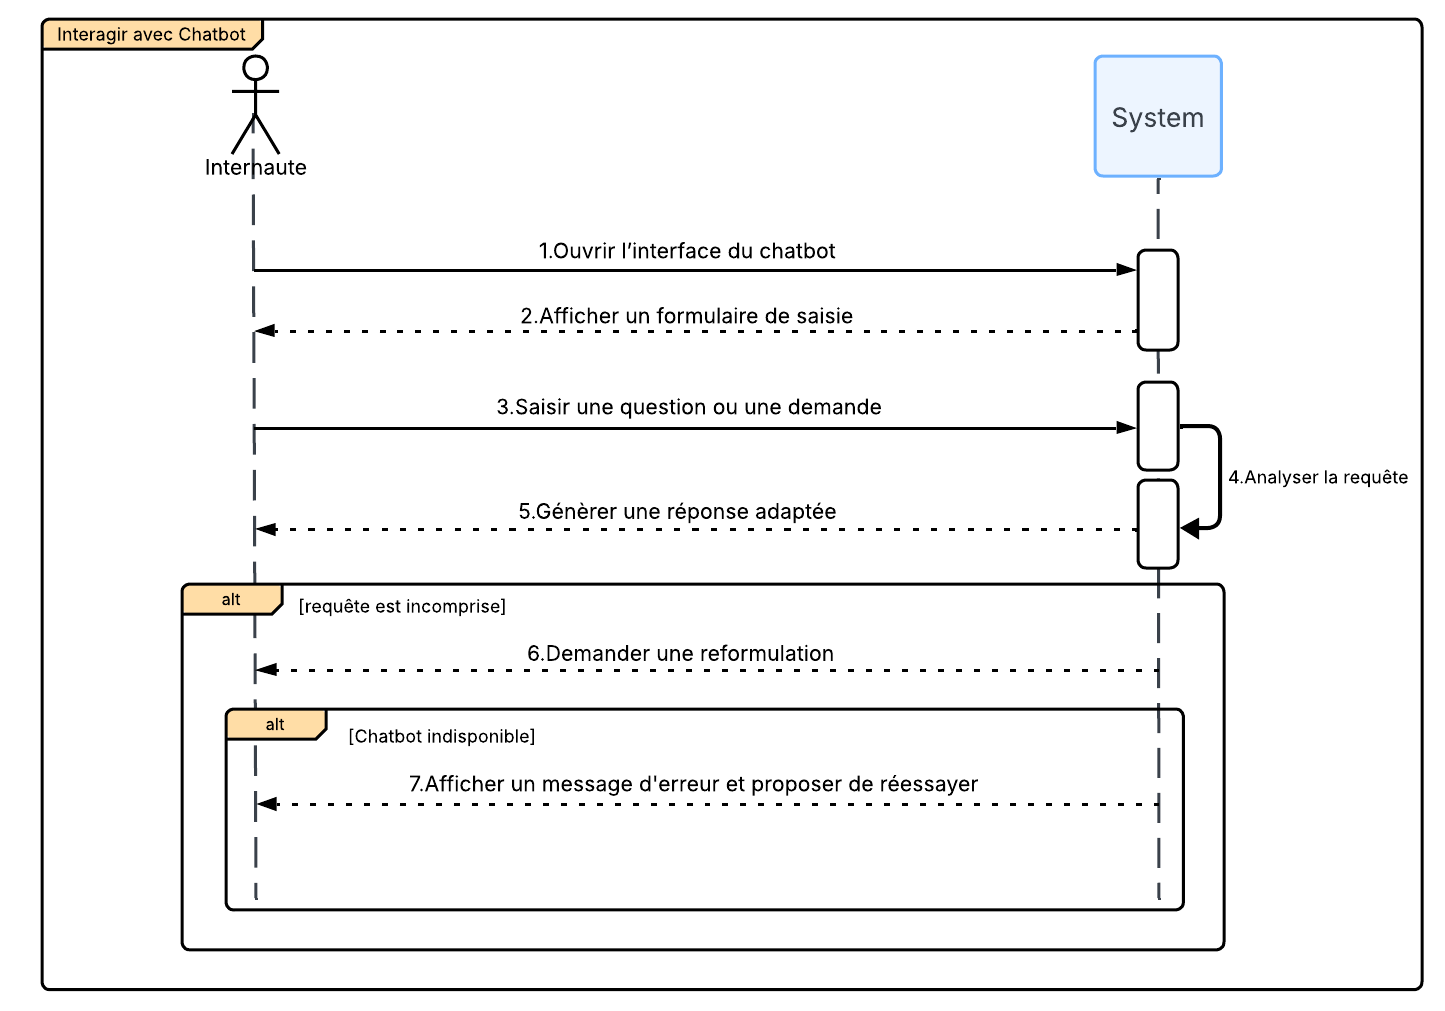
\includegraphics[width=0.7\textwidth]{Chapitres/Figures/Diag_seq_chatbot.png}
    \caption{Diagramme de séquence système de cas d'utilisation «Interagir avec Chatbot»}
    \label{fig:chatbot}
\end{figure}

%==========================================================
\section{Analyse des cas d'utilisation de l'acteur "Utilisateur''}
\label{sec:acteur_utilisateur_s2}

\subsection{Analyse de cas d'utilisation "Voir score client''}
\label{sec:voir_score}

La section suivante présente l'analyse du cas d'utilisation "Voir score client''
de l'acteur utilisateur.

\begin{table}[H]
\centering
\caption{Description textuelle du cas d'utilisation "Voir score client''}
\label{tab:voir_score}
\renewcommand{\arraystretch}{1.35}
\begin{tabular}{|p{3.5cm}|p{10cm}|}
\hline
\textbf{Élément} & \textbf{Description} \\
\hline
Nom & Voir score client \\
\hline
Acteur & Utilisateur \\
\hline
Description brève & Permet à l'utilisateur de consulter le score de fiabilité calculé automatiquement à partir de son historique de location. \\
\hline
Précondition & L'utilisateur est authentifié. \newline
               Le système est accessible. \\
\hline
Postcondition & Le score de fiabilité de l'utilisateur est affiché ainsi que les critères ayant contribué à son calcul. \\
\hline
Enchaînement principal &
1. L'utilisateur accède à son espace personnel. \newline
2. Le système calcule le score à partir de l'historique (retards, annulations, incidents). \newline
3. Le système affiche le score de fiabilité ainsi que son détail. \\
\hline
\textbf{Scénario alternatif} &
2.1 Historique insuffisant pour calculer un score. \newline
\quad 2.1.1 Le système affiche un score par défaut "100''. \newline
2.2 Erreur de calcul. \newline
\quad 2.2.1 Le système affiche un message d'erreur. \\
\hline
\end{tabular}
\end{table}

\begin{figure}[H]
    \centering
    
\includegraphics[width=0.7\textwidth]{Chapitres/figures/diag_seq_voir_score_client.png}
    \caption{Diagramme de séquence système de cas d'utilisation "Voir score client''}
    \label{fig:seq_voir_score}
\end{figure}


\section{Analyse des cas d'utilisation de l'acteur "Client''}
\label{sec:acteur_client_s2}

%----------------------------------------------------------
\subsection{Analyse de cas d'utilisation "Effectuer réservation''}
\label{sec:effectuer_reservation}

Afin de mieux illustrer le déroulement du scénario, nous proposons ci-après une
description textuelle accompagnée du diagramme de séquence du cas d'utilisation
"\textbf{Effectuer réservation}''.

\begin{table}[H]
\centering
\caption{Description textuelle du cas d'utilisation "Effectuer réservation''}
\label{tab:effectuer_reservation}
\renewcommand{\arraystretch}{1.35}
\begin{tabular}{|p{3.5cm}|p{10cm}|}
\hline
\textbf{Élément} & \textbf{Description} \\
\hline
Nom & Effectuer réservation \\
\hline
Acteur & Client \\
\hline
Description brève & Permet au client de réserver une voiture disponible pour une période déterminée. \\
\hline
Précondition & Le client est authentifié. \newline
               Le système est accessible. \newline
               Au moins un véhicule est disponible. \\
\hline
Postcondition & La réservation est enregistrée et son statut est "~En attente~''. \newline
                Le client reçoit une confirmation de sa demande. \\
\hline
Enchaînement principal &
1. Le client choisit une voiture à réserver.\newline
2. Le système affiche les détails de la voiture.\newline
3. Le client demande une réservation.\newline
4. Le système affiche le formulaire de saisie des informations de réservation.\newline
5. Le client saisit les informations de réservation (date, jours).\newline
6. Le système vérifie les informations saisies.\newline
7. Le système vérifie la disponibilité de la voiture.\newline
8. Le système affiche un message de confirmation de réservation.\\
\hline
\textbf{Scénario alternatif} &
6.1 Champs incomplets.\newline
\quad 6.1.1 Le système affiche un message d'erreur.\newline
7.1 Voiture indisponible.\newline
\quad 7.1.1 Le système affiche le message « La voiture est réservée pour la date saisie ».\\
\hline
\end{tabular}
\end{table}

\begin{figure}[H]
    \centering
    
\includegraphics[width=0.8\textwidth]{Chapitres/figures/Diag_seq_effectuer_reservation.png}
    \caption{Diagramme de séquence système de cas d'utilisation "Effectuer réservation''}
    \label{fig:seq_effectuer_reservation}
\end{figure}

%----------------------------------------------------------
\newpage
\subsection{Analyse de cas d'utilisation "Consulter réservations en cours''}
\label{sec:consulter_reservations}

Afin de mieux illustrer le déroulement du scénario, nous proposons ci-après une
description textuelle accompagnée du diagramme de séquence du cas d'utilisation
"\textbf{Consulter réservations en cours}''.

\begin{table}[H]
\centering
\caption{Description textuelle du cas d'utilisation "Consulter réservations en cours''}
\label{tab:consulter_reservations}
\renewcommand{\arraystretch}{1.35}
\begin{tabular}{|p{3.5cm}|p{10cm}|}
\hline
\textbf{Élément} & \textbf{Description} \\
\hline
Nom & Consulter réservations en cours \\
\hline
Acteur & Client \\
\hline
Description brève & Permet au client de consulter l'état de ses réservations actives. \\
\hline
Précondition & Le client est authentifié. \newline
               Le système est accessible. \\
\hline
Postcondition & La liste des réservations en cours est affichée avec leur statut respectif. \\
\hline
Enchaînement principal &
1. Le client accède à la section "Mes réservations''. \newline
2. Le système récupère les réservations associées au compte client. \newline
3. Le système affiche la liste des réservations avec leur statut (En attente, Confirmée, En cours, Terminée). \newline
4. Le client sélectionne une réservation pour consulter les détails. \newline
5. Le système affiche les informations détaillées de la réservation. \\
\hline
\textbf{Scénario alternatif} &
Pas d'exceptions \\
\hline
\end{tabular}
\end{table}

\begin{figure}[H]
    \centering
    
\includegraphics[width=0.8\textwidth]{Chapitres/figures/diag_seq_consulter_reservations_en_cours.png}
    \caption{Diagramme de séquence système de cas d'utilisation "Consulter réservations en cours''}
    \label{fig:seq_consulter_reservations}
\end{figure}

%==========================================================
\section{Analyse des cas d'utilisation de l'acteur "Agence''}
\label{sec:acteur_agence_s2}

%----------------------------------------------------------
\subsection{Analyse de cas d'utilisation "Traiter réservations''}
\label{sec:traiter_reservations}

Pour mieux analyser le déroulement du scénario, nous proposons ci-après une description textuelle et un diagramme de séquence du cas
d'utilisation "\textbf{Traiter réservations}'' de l'acteur Agence.

\begin{table}[H]
\centering
\caption{Description textuelle du cas d'utilisation "Traiter réservations''}
\label{tab:traiter_reservations}
\renewcommand{\arraystretch}{1.35}
\begin{tabular}{|p{3.5cm}|p{10cm}|}
\hline
\textbf{Élément} & \textbf{Description} \\
\hline
Nom & Traiter réservations \\
\hline
Acteur & Agence \\
\hline
Description brève & Permet à l'agence de consulter, accepter ou refuser les demandes de réservation des clients. \\
\hline
Précondition & L'agence est authentifiée. \newline
               Des demandes de réservation existent dans le système. \\
\hline
Postcondition & La réservation est acceptée ou refusée. \newline
                Le statut de la réservation est mis à jour. \newline
                Le client est notifié de la décision. \\
\hline
Enchaînement principal &
1. L'agence consulte les demandes de réservations. \newline
2. Le système affiche la liste des demandes. \newline
3. L'agence sélectionne une demande. \newline
4. L'agence choisit d'accepter la réservation. \newline
5. Le système met à jour le statut de la réservation. \newline
6. Le système affiche un message "Réservation acceptée''. \newline
7. Le système envoie une notification d'acceptation au client. \\
\hline
\textbf{Scénario alternatif} &
4.1 Refus de la réservation. \newline
\quad 4.1.1 L'agence choisit de refuser la demande. \newline
\quad 4.1.2 Le système confirme le refus. \newline
\quad 4.1.3 Le système envoie une notification de refus au client. \\
\hline
\end{tabular}
\end{table}

\begin{figure}[H]
    \centering
    
\includegraphics[width=1\textwidth]{Chapitres/figures/seq_traiter_reservation.png}
    \caption{Diagramme de séquence système de cas d'utilisation "Traiter réservations''}
    \label{fig:seq_traiter_reservation}
\end{figure}

%----------------------------------------------------------
\subsection{Analyse de cas d'utilisation "Consulter statistiques-Agence''}
\label{sec:stats_agence}

Dans la suite, nous présentons une description textuelle accompagnée d'un diagramme
de séquence du cas d'utilisation "\textbf{Consulter statistiques}'' de l'acteur Agence.

\begin{table}[H]
\centering
\caption{Description textuelle du cas d'utilisation "Consulter statistiques-Agence''}
\label{tab:stats_agence}
\renewcommand{\arraystretch}{1.35}
\begin{tabular}{|p{3.5cm}|p{10cm}|}
\hline
\textbf{Élément} & \textbf{Description} \\
\hline
Nom & Consulter statistiques \\
\hline
Acteur & Agence \\
\hline
Description brève & Permet à l'agence de visualiser ses indicateurs de performance à travers un tableau de bord interactif. \\
\hline
Précondition & L'agence est authentifiée. \newline
               Le système est accessible. \\
\hline
Postcondition & Les indicateurs de performance sont affichés (nombre de réservations, taux d'occupation, chiffre d'affaires, satisfaction client). \\
\hline
Enchaînement principal &
1. L'agence accède à "~Statistiques~''. \newline
2. Le système collecte les données relatives à l'activité de l'agence. \newline
3. Le système génère et affiche les indicateurs clés (graphiques, tableaux, synthèses). \newline
4. L'agence consulte et analyse les données. \\
\hline
\textbf{Scénario alternatif} &
Pas d'exceptions \\
\hline
\end{tabular}
\end{table}

\begin{figure}[H]
    \centering
    
\includegraphics[width=1\textwidth]{Chapitres/figures/seq_stats_agence.png}
    \caption{Diagramme de séquence système de cas d'utilisation "Consulter statistiques-Agence''}
    \label{fig:seq_stats_agence}
\end{figure}

%==========================================================
\section{Analyse des cas d'utilisation de l'acteur "Administrateur''}
\label{sec:acteur_admin_s2}

%----------------------------------------------------------

%----------------------------------------------------------
\subsection{Analyse de cas d'utilisation "Consulter statistiques-Administrateur''}
\label{sec:stats_admin}

Dans la suite, nous présentons une description textuelle accompagnée d'un diagramme
de séquence du cas d'utilisation "\textbf{Consulter statistiques globales}'' de
l'acteur Administrateur.

\begin{table}[H]
\centering
\caption{Description textuelle du cas d'utilisation "Consulter statistiques-Administrateur''}
\label{tab:stats_admin}
\renewcommand{\arraystretch}{1.35}
\begin{tabular}{|p{3.5cm}|p{10cm}|}
\hline
\textbf{Élément} & \textbf{Description} \\
\hline
Nom & Consulter statistiques globales \\
\hline
Acteur & Administrateur \\
\hline
Description brève & Permet à l'administrateur de visualiser les indicateurs de performance globaux de l'ensemble de la plateforme afin de détecter les anomalies et d'améliorer le système. \\
\hline
Précondition & L'administrateur est authentifié. \newline
               Le système est accessible. \\
\hline
Postcondition & Les indicateurs globaux sont affichés (nombre total d'agences, de réservations, de clients, score moyen, anomalies détectées). \\
\hline
Enchaînement principal &
1. L'administrateur accède à"~Statistiques~''. \newline
2. Le système collecte les données globales de toutes les agences. \newline
3. Le système génère et affiche les indicateurs clés de performance (KPI). \newline
4. L'administrateur consulte les données. \newline
5. L'administrateur peut filtrer les données par période ou par agence. \\
\hline
\textbf{Scénario alternatif} &
Pas d'exceptions \\
\hline
\end{tabular}
\end{table}

\begin{figure}[H]
    \centering
    
\includegraphics[width=1\textwidth]{Chapitres/figures/seq_stats_admin.png}
    \caption{Diagramme de séquence système de cas d'utilisation "Consulter statistiques-Administrateur''}
    \label{fig:seq_stats_admin}
\end{figure}

%----------------------------------------------------------

\section{Diagramme de classe du deuxième sprint}
\label{sec:sec_diag_classe_sprint_2}

\begin{figure}[H]
    \centering
    
\includegraphics[width=1\textwidth]{Chapitres/figures/Diag_classe_sprint_2.png}
    \caption{Diagramme de classe du deuxième sprint}
    \label{fig:classe_sprint2}
\end{figure}

%==========================================================
\section{Conception des cas d'utilisation}
\label{sec:conception_s2}

Nous illustrerons dans cette section la conception de ce deuxième sprint à travers
la réalisation d'un diagramme des classes pour chaque module, ainsi que d'un
diagramme de séquence détaillé correspondant à chaque cas d'utilisation analysé.

%==========================================================
\subsection{Diagramme des classes participantes}
\label{sec:classes_participantes_s2}


\subsubsection{Diagramme des classes participantes par acteur "Utilisateur''}
\label{Diag_classes_participantes_utilisateur_s2}
\begin{figure}[H]
    \centering
    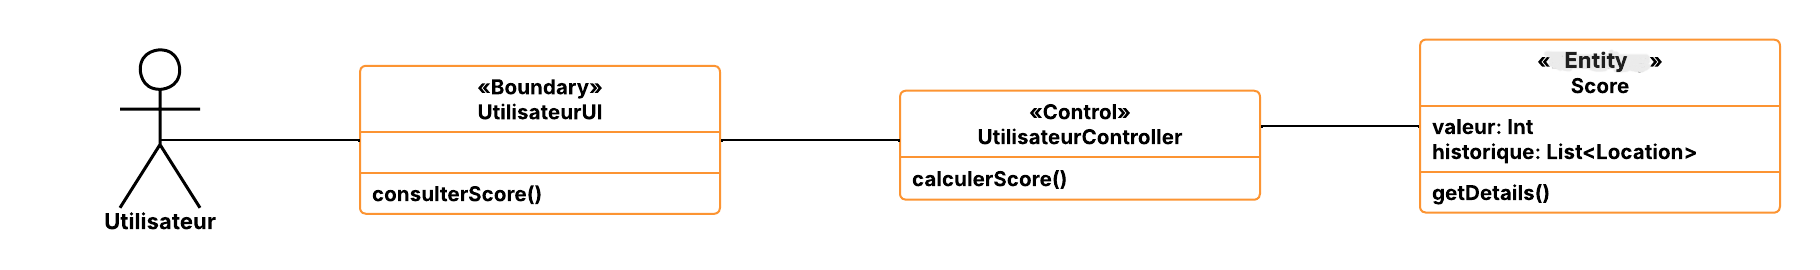
\includegraphics[width=1\textwidth]{Chapitres/Figures/classes_participantes__utilisateur_s2.png}
    \caption{Diagramme des classes participantes par acteur Utilisateur}
    \label{fig:classes_participantes_utilisateur_s2}
\end{figure}

\subsubsection{Diagramme des classes participantes par acteur "Client''}
\label{Diag_classes_participantes_client_s2}
\begin{figure}[H]
    \centering
    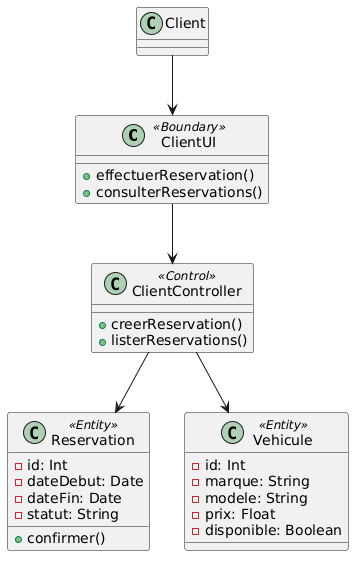
\includegraphics[width=1\textwidth]{Chapitres/Figures/classes_participantes__client_s2.png}
    \caption{Diagramme des classes participantes par acteur Client}
    \label{fig:classes_participantes_client_s2}
\end{figure}

\subsubsection{Diagramme des classes participantes par acteur "Agence''}
\label{Diag_classes_participantes_agence_s2}
\begin{figure}[H]
    \centering
    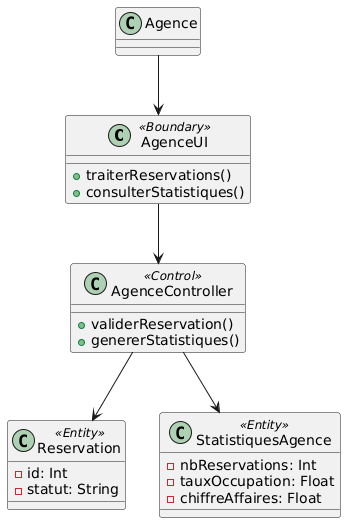
\includegraphics[width=1\textwidth]{Chapitres/Figures/classes_participantes__agence_s2.png}
    \caption{Diagramme des classes participantes par acteur Agence}
    \label{fig:classes_participantes_agence_s2}
\end{figure}

\subsubsection{Diagramme des classes participantes par acteur "Administrateur''}
\label{Diag_classes_participantes_administrateur_s2}
\begin{figure}[H]
    \centering
    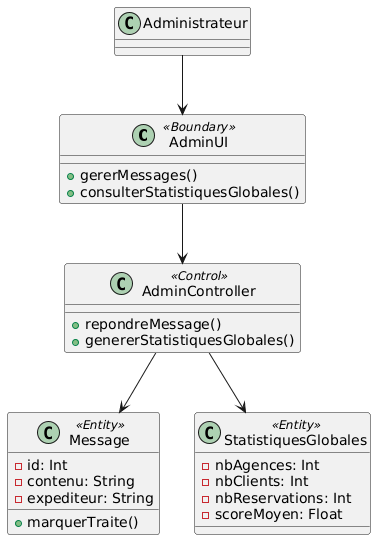
\includegraphics[width=1\textwidth]{Chapitres/Figures/classes_participantes__admin_s2.png}
    \caption{Diagramme des classes participantes par acteur Administrateur}
    \label{fig:classes_participantes_admin_s2}
\end{figure}
%%%%%%%%%%%%%%%%%%%%%%seq_détaillée%%%%%%%%%%%%%%%%%%%%%%%%%%%%%%%%%%%%%%%%%%%%%%%%%%%%%%%%%%%%%%%%%%%%%%%%%%%%%%%
\section{Diagrammes de séquence détaillés du deuxiéme sprint}
\label{sec:diag_seq_detail_s2}

%====================================================
\subsection{Diagrammes de séquence détaillés de l’acteur Utilisateur}
\label{sec:diag_seq_utilisateur_s2}

\subsubsection{Diagrammes de séquence détaillé du cas d’utilisation " Voir score client ''}
\label{sec:diag_seq_det_score_client}
\begin{figure}[H]
    \centering
    
\includegraphics[width=0.85\textwidth]{Chapitres/figures/diag_seq_det/seq_det_s2/seq_det_score_client.png}
    \caption{Diagramme de séquence détaillé du cas d’utilisation " Voir score client ''}
    \label{fig:seq_det_score_client}
\end{figure}

%====================================================
\subsection{Diagrammes de séquence détaillés de l’acteur Client}
\label{sec:diag_seq_client_s2}

\subsubsection{Diagrammes de séquence détaillé du cas d’utilisation " Effectuer réservation ''}
\label{sec:diag_seq_det_effectuer_reservation}
\begin{figure}[H]
    \centering
    
\includegraphics[width=0.95\textwidth]{Chapitres/figures/diag_seq_det/seq_det_s2/seq_det_effectuer_reservation.png}
    \caption{Diagramme de séquence détaillé du cas d’utilisation " Effectuer réservation ''}
    \label{fig:seq_det_effectuer_reservation}
\end{figure}

\subsubsection{Diagrammes de séquence détaillé du cas d’utilisation " Consulter reservation ''}
\label{sec:diag_seq_det_consulter_reservation}
\begin{figure}[H]
    \centering
    
\includegraphics[width=0.9\textwidth]{Chapitres/figures/diag_seq_det/seq_det_s2/seq_det_consulter_reservation.png}
    \caption{Diagramme de séquence détaillé du cas d’utilisation " Consulter réservations en cours ''}
    \label{fig:seq_det_consulter_reservation}
\end{figure}

%====================================================
\subsection{Diagrammes de séquence détaillés de l’acteur Agence}
\label{sec:diag_seq_agence_s2}

\subsubsection{Diagrammes de séquence détaillé du cas d’utilisation " Traiter réservations ''}
\label{sec:diag_seq_det_traiter_reservations}
\begin{figure}[H]
    \centering
    
\includegraphics[width=0.95\textwidth]{Chapitres/figures/diag_seq_det/seq_det_s2/seq_det_traiter_reservations.png}
    \caption{Diagramme de séquence détaillé du cas d’utilisation " Traiter réservations ''}
    \label{fig:seq_det_traiter_reservations}
\end{figure}

\subsubsection{Diagrammes de séquence détaillé du cas d’utilisation " Consulter statistiques agence ''}
\label{sec:diag_seq_det_Consulter_statistiques_agence}
\begin{figure}[H]
    \centering
    
\includegraphics[width=0.85\textwidth]{Chapitres/figures/diag_seq_det/seq_det_s2/seq_det_stat_agence.png}
    \caption{Diagramme de séquence détaillé du cas d’utilisation " Consulter statistiques agence ''}
    \label{fig:seq_det_stat_agence}
\end{figure}

%====================================================
\subsection{Diagrammes de séquence détaillés de l’acteur Administrateur}
\label{sec:diag_seq_admin_s2}

\subsubsection{Diagrammes de séquence détaillé du cas d’utilisation " Gérer messages ''}
\label{sec:diag_seq_det_gerer_message}
\begin{figure}[H]
    \centering
    
\includegraphics[width=0.9\textwidth]{Chapitres/figures/diag_seq_det/seq_det_s2/seq_det_gerer_messages.png}
    \caption{Diagramme de séquence détaillé du cas d’utilisation " Gérer messages ''}
    \label{fig:seq_det_gerer_messages}
\end{figure}

\subsubsection{Diagrammes de séquence détaillé du cas d’utilisation " Consulter statistiques administrateur ''}
\label{sec:diag_seq_det_stat_admin}
\begin{figure}[H]
    \centering
    
\includegraphics[width=0.85\textwidth]{Chapitres/figures/diag_seq_det/seq_det_s2/seq_det_stat_admin.png}
    \caption{Diagramme de séquence détaillé du cas d’utilisation " Consulter statistiques administrateur ''}
    \label{fig:seq_det_stat_admin}
\end{figure}
%%%%%%%%%%%%%%%%%%%%%%%%%%%%%%%%%%%%%%%%%%%%%%%%%%%%%%%%%%%%%%%%%%%%%%%%%%%%%%%%%%%%%%%%%%%%%%%%%%%%%%%%%%%%%%%%%%
%----------------------------------------------------------

\section{Diagramme de classe du deuxième sprint}
\label{sec:sec_diag_classe_sprint2}

\begin{figure}[H]
    \centering
    
\includegraphics[width=1\textwidth]{Chapitres/figures/Diag_classe_sprint_2.png}
    \caption{Diagramme de classe du deuxième sprint}
    \label{fig:diag_classe_sprint2}
\end{figure}

\section{Implémentation}
\label{sec:implementation_s2}

Le module d'implémentation du deuxième sprint présente la mise en œuvre technique des fonctionnalités développées, en détaillant leur réalisation au niveau du code et leur intégration dans l'application.

\subsection{Tables de la base de données}
\subsubsection{Tableau « reservations »}
\begin{table}[H]
\centering
\caption{Tableau « reservations »}
\label{tab:reservations}
\renewcommand{\arraystretch}{1.3}
\resizebox{\textwidth}{!}{%
\begin{tabular}{|l|l|p{4cm}|l|}
\hline
\textbf{Champs} & \textbf{Type} & \textbf{Libellé} & \textbf{Contraintes} \\
\hline
id & BigInt UNSIGNED & Identifiant unique de la réservation & PRIMARY KEY, AUTO\_INCREMENT, NOT NULL \\
\hline
user\_id & BigInt UNSIGNED & Identifiant du client & FOREIGN KEY (users), NOT NULL \\
\hline
vehicle\_id & BigInt UNSIGNED & Identifiant du véhicule & FOREIGN KEY (vehicles), NOT NULL \\
\hline
start\_date & Date & Date de début de location & NOT NULL \\
\hline
end\_date & Date & Date de fin de location & NOT NULL \\
\hline
pickup\_location & Varchar(255) & Lieu de récupération & NULLABLE \\
\hline
dropoff\_location & Varchar(255) & Lieu de retour & NULLABLE \\
\hline
base\_price & Decimal(10,2) & Coût base de location & NOT NULL \\
\hline
discount\_amount & Decimal(10,2) & Montant remise appliquée & NOT NULL, DEFAULT 0.00 \\
\hline
additional\_charges & Decimal(10,2) & Frais supplémentaires & NOT NULL, DEFAULT 0.00 \\
\hline
total\_price & Decimal(10,2) & Prix total à payer & NOT NULL \\
\hline
platform\_commission\_rate & Decimal(5,4) & Taux commission plateforme & NOT NULL, DEFAULT 0.0800 \\
\hline
platform\_commission & Decimal(10,2) & Commission plateforme & NOT NULL, DEFAULT 0.00 \\
\hline
agency\_payout & Decimal(10,2) & Paiement agence & NOT NULL, DEFAULT 0.00 \\
\hline
paid\_amount & Decimal(10,2) & Montant déjà payé & NOT NULL, DEFAULT 0.00 \\
\hline
remaining\_amount & Decimal(10,2) & Solde impayé & NOT NULL, DEFAULT 0.00 \\
\hline
\end{tabular}%
}
\end{table}


Le tableau suivant présente le dictionnaire des données du deuxième sprint, en précisant pour chaque table les attributs définis, leurs libellés ainsi que leurs types.

\subsubsection{Tableau « contact\_messages »}
\begin{table}[H]
\centering
\caption{Tableau « contact\_messages »}
\label{tab:contact_messages}
\renewcommand{\arraystretch}{1.3}
\resizebox{\textwidth}{!}{%
\begin{tabular}{|l|l|p{4cm}|l|}
\hline
\textbf{Champs} & \textbf{Type} & \textbf{Libellé} & \textbf{Contraintes} \\
\hline
id & BigInt UNSIGNED & Identifiant unique du message & PRIMARY KEY, AUTO\_INCREMENT, NOT NULL \\
\hline
name & Varchar(255) & Nom du contact & NOT NULL \\
\hline
email & Varchar(255) & Email du contact & NOT NULL \\
\hline
phone & Varchar(255) & Numéro téléphone & NULLABLE \\
\hline
subject & Varchar(255) & Sujet du message & NOT NULL \\
\hline
message & Text & Corps du message & NOT NULL \\
\hline
admin\_reply & Text & Réponse de l'admin (snapshot) & NULLABLE \\
\hline
replied\_by\_email & Varchar(255) & Email de l'admin qui répond & NULLABLE \\
\hline
replied\_at & Timestamp & Date de réponse & NULLABLE \\
\hline
is\_read & TinyInt(1) & Message lu & NOT NULL, DEFAULT 0 \\
\hline
submitted\_at & Timestamp & Date de soumission & NULLABLE \\
\hline
read\_at & Timestamp & Date de lecture & NULLABLE \\
\hline
created\_at & Timestamp & Date de création & NULLABLE \\
\hline
updated\_at & Timestamp & Date de modification & NULLABLE \\
\hline
\end{tabular}%
}
\end{table}

\subsubsection{Tableau « client\_reliability\_scores »}
\begin{table}[H]
\centering
\caption{Tableau « client\_reliability\_scores »}
\label{tab:client_reliability_scores}
\renewcommand{\arraystretch}{1.3}
\resizebox{\textwidth}{!}{%
\begin{tabular}{|l|l|p{4cm}|l|}
\hline
\textbf{Champs} & \textbf{Type} & \textbf{Libellé} & \textbf{Contraintes} \\
\hline
id & BigInt UNSIGNED & Identifiant unique du score & PRIMARY KEY, AUTO\_INCREMENT, NOT NULL \\
\hline
user\_id & BigInt UNSIGNED & Identifiant du client & FOREIGN KEY (users), NOT NULL \\
\hline
total\_reservations & Int & Nombre total de réservations & NOT NULL, DEFAULT 0 \\
\hline
completed\_reservations & Int & Réservations complétées & NOT NULL, DEFAULT 0 \\
\hline
cancelled\_reservations & Int & Réservations annulées & NOT NULL, DEFAULT 0 \\
\hline
late\_returns & Int & Retours en retard & NOT NULL, DEFAULT 0 \\
\hline
payment\_delays & Int & Retards de paiement & NOT NULL, DEFAULT 0 \\
\hline
damage\_incidents & Int & Incidents dommages & NOT NULL, DEFAULT 0 \\
\hline
total\_unpaid\_amount & Decimal(10,2) & Solde impayé total & NOT NULL, DEFAULT 0.00 \\
\hline
reliability\_score & Int & Score fiabilité (0-100) & NOT NULL, DEFAULT 100 \\
\hline
risk\_level & Enum('low','medium','high','blocked') & Niveau risque & NOT NULL, DEFAULT 'low' \\
\hline
admin\_notes & Text & Notes administrateur & NULLABLE \\
\hline
last\_calculated\_at & Timestamp & Dernière recalculation & NULLABLE \\
\hline
created\_at & Timestamp & Date de création & NULLABLE \\
\hline
updated\_at & Timestamp & Date de modification & NULLABLE \\
\hline
\end{tabular}%
}
\end{table}

\subsection{Réalisation des interfaces du deuxième sprint}

Nous présentons dans cette section les interfaces graphiques développées lors du deuxième sprint.


\subsubsection{Interface contact administrateur :}

\begin{figure}[H]
    \centering
    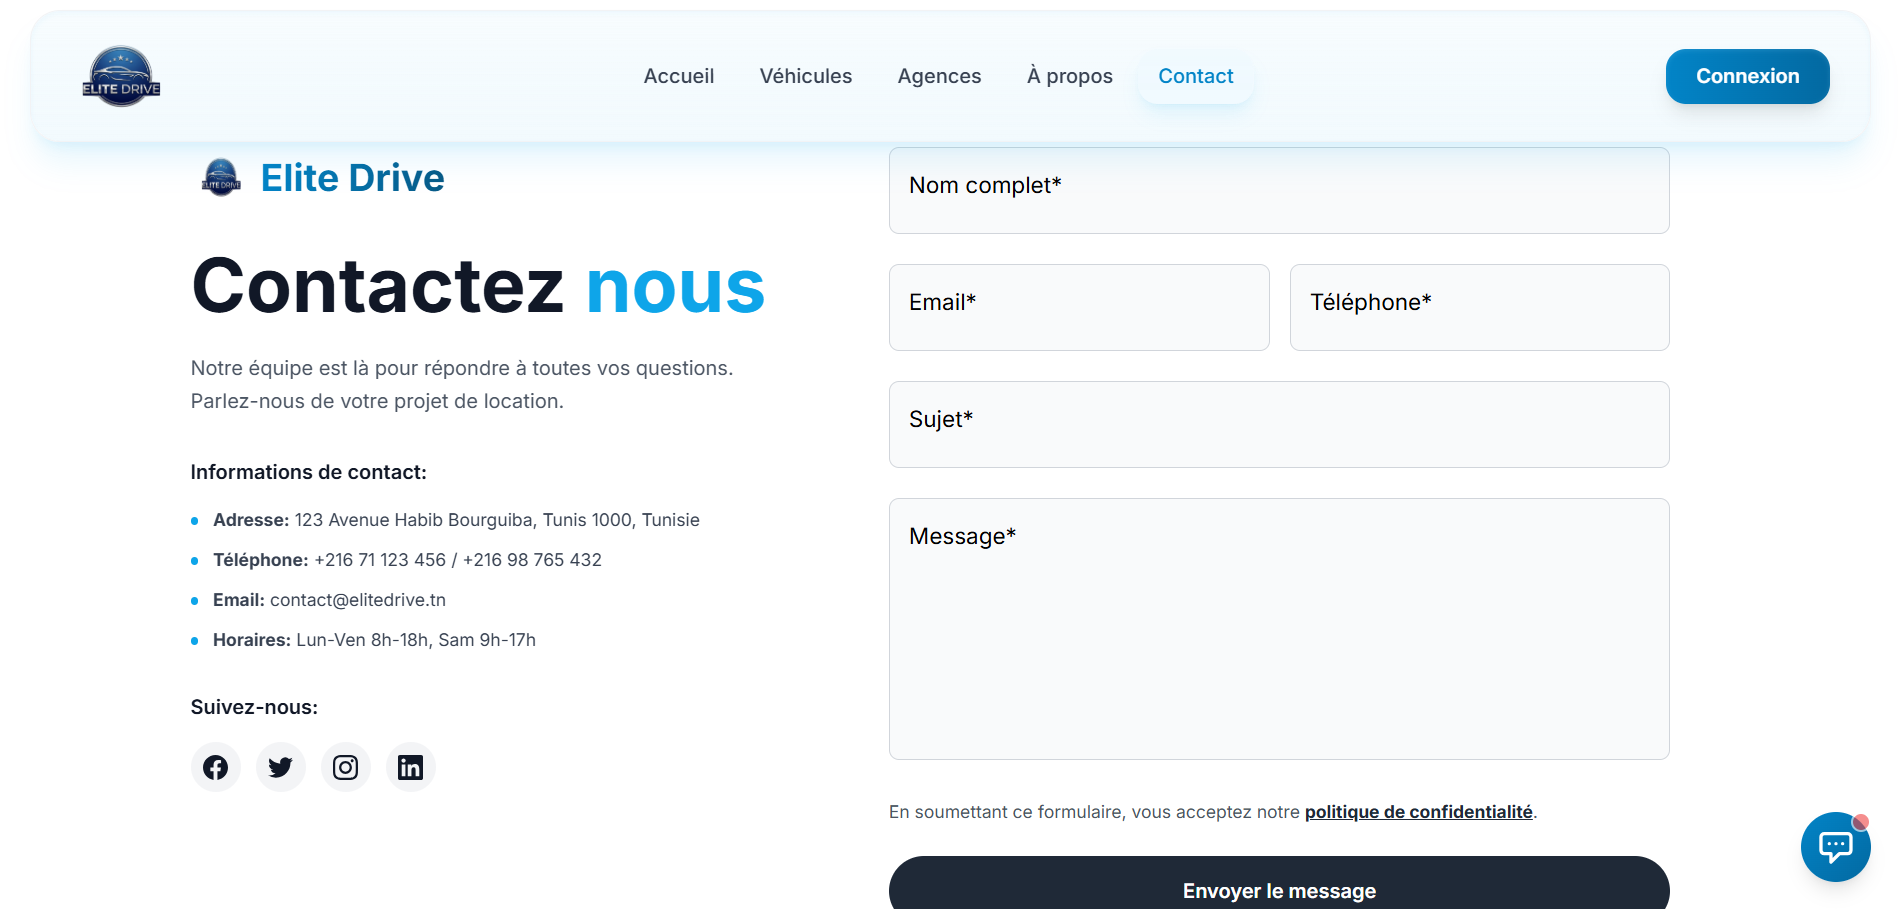
\includegraphics[width=0.9\linewidth]{Chapitres/Figures/inter_contact.png}    
    \caption{Interface contact administrateur}
    \label{fig:interface_contact_admin_s2}
\end{figure}


\subsubsection{Interface formulaire réservation :}

\begin{figure}[H]
    \centering
    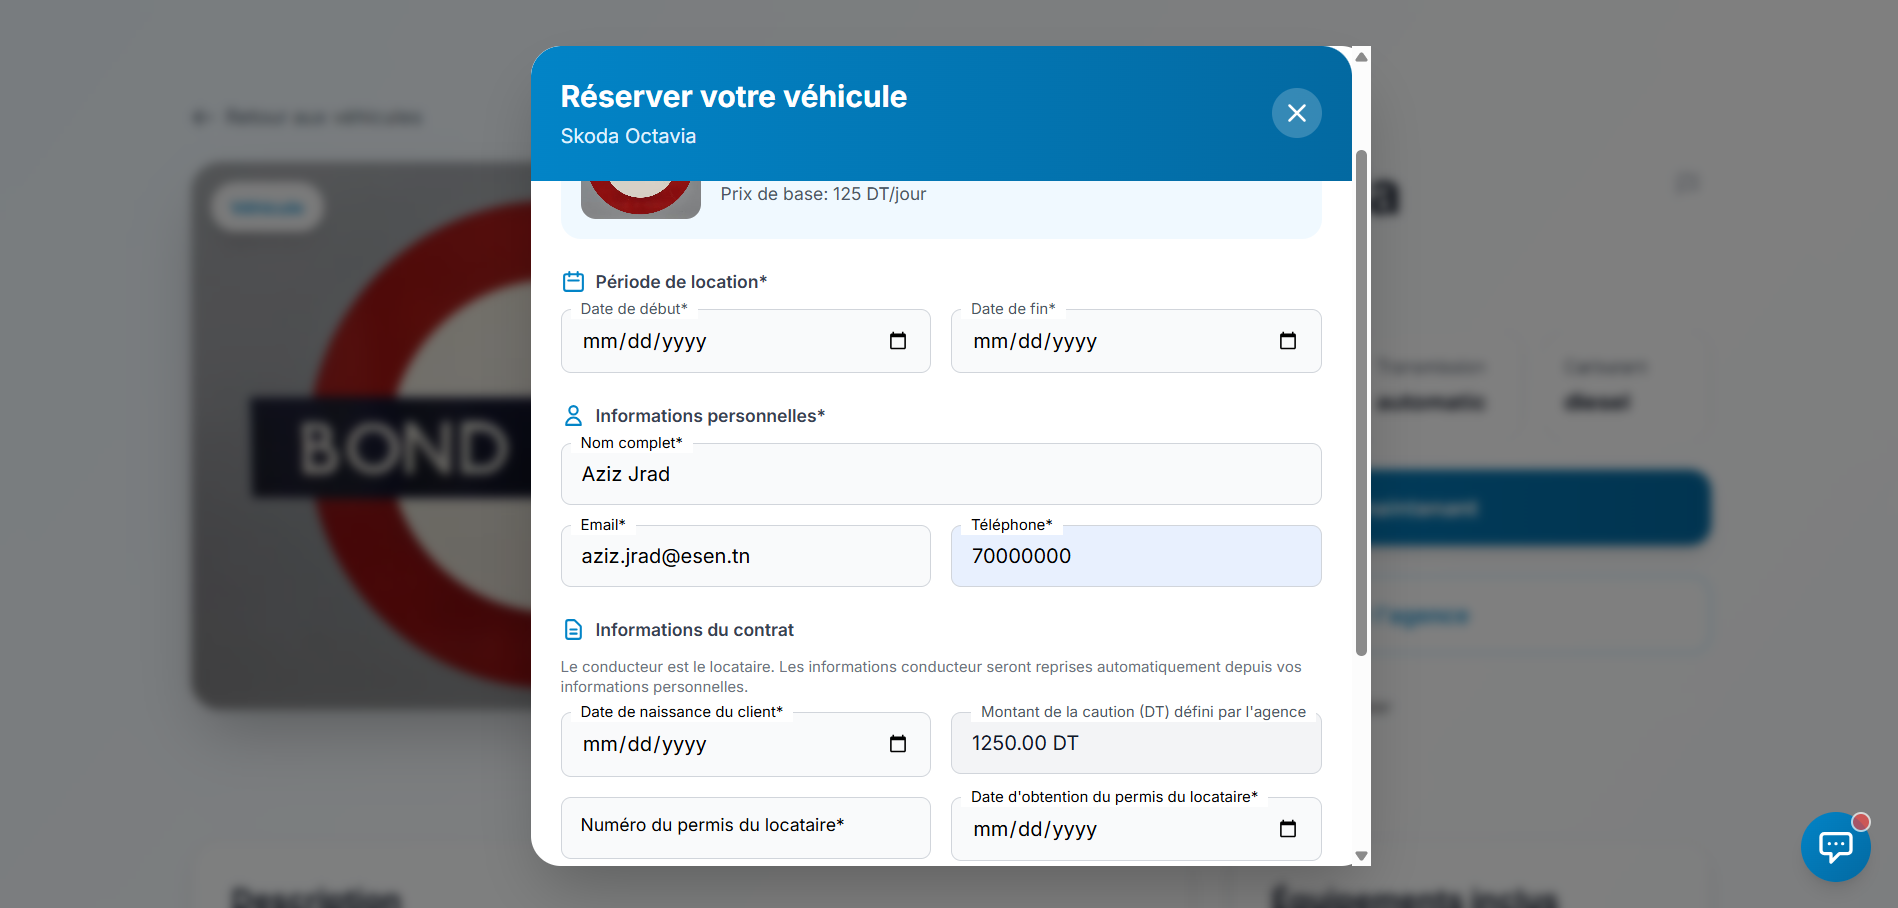
\includegraphics[width=0.9\linewidth]{Chapitres/Figures/inter_reservation.png}
    \caption{Interface réservation}
    \label{fig:interface_reservation_s2}
\end{figure}


\subsubsection{Interface statistiques globales :}

\begin{figure}[H]
    \centering
    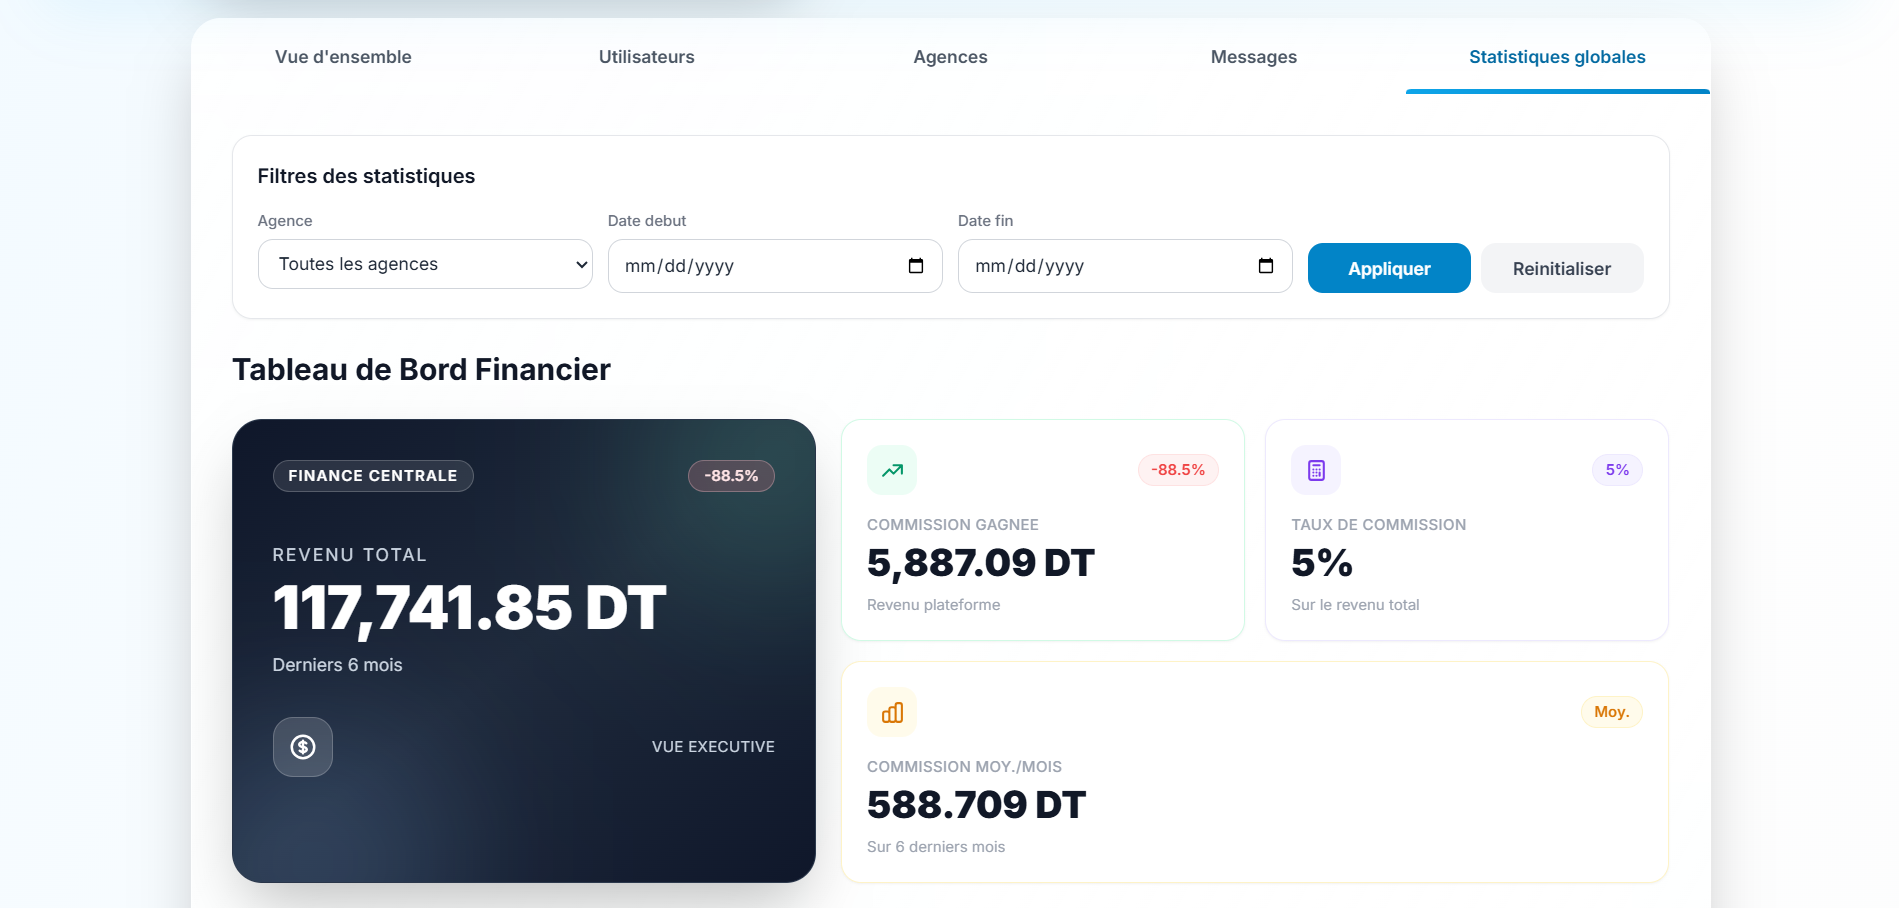
\includegraphics[width=0.9\linewidth]{Chapitres/Figures/inter_statsglobal.png}
    \caption{Interface statistiques globales}
    \label{fig:interface statistiques globales_s2}
\end{figure}



%----------------------------------------------------------
\section{Test}
\label{sec:test_sprint2}

\subsection{Test unitaire}
\label{sec:test_unitaire_s2}

\subsubsection{Test unitaire du cas d'utilisation "Voir score client''}

Cette section se concentre sur la reprise d'une partie du code pour le cas "Voir score client''.

\subsubsection*{--- Code source du cas d'utilisation "Voir score client''}

\begin{figure}[H]
    \centering
    
\includegraphics[width=0.9\textwidth]{Chapitres/figures/score_test.png}
    \caption{Test unitaire du cas d'utilisation "Voir score client''}
    \label{fig:test_unitaire_voir_score_client}
\end{figure}

%----------------------------------------------------------
\section{Conclusion}
\label{sec:conclusion_sprint2}

Dans le cadre de ce chapitre, nous avons mené le Sprint~2 selon une séquence logique
couvrant l'analyse des cas d'utilisation et la conception. Les fonctionnalités
développées — effectuer et suivre des réservations, visualiser le score de fiabilité,
traiter les réclamations, consulter les statistiques et gérer les messages — constituent
le cœur métier de la plateforme et assurent une expérience complète pour l'ensemble
des acteurs du système.

La phase suivante sera consacrée à la présentation des résultats obtenus, des
technologies utilisées, ainsi qu'au déploiement de la solution.
